\section{緒言}
\subsection{緒言}
現在,関節を多様にデザインする研究が盛んにおこなわれており,本研究では紐で構成される関節に注目する.この関節はリンクの間を紐でつなぐ構造であり,本論文では紐関節と呼ぶ.紐関節は,紐の配置方法や長さによって異方性を持たせることができ,同一の構造でありながら屈曲方向や剛性の異なる関節を再現できる.また,紐のみで関節を製造するため低コストである.ここで,図\ref{紐関節}に製造対象となる紐関節を示す.この紐関節はリンク表面に紐を接着し,紐のたるみを利用したものである.図\ref{紐関節}の関節を製造するためには関節の異なる長さの紐を接続する必要がある.しかし,製造過程で紐に想定していないねじれやたるみが起こることや,紐を切断しその後の紐を安定して制御することは難しい.そのため,製造手法が確立されていない\cite{山本圭治郎2012}.
\par
前述した課題を解決するために,本研究では1つ目に,紐の切断を省略し,1本の紐で関節を製造する手法を提案する.その前段階として,異なる長さの紐のたるみを制御し接続する手法を確立する.2つ目に,紐関節を製造するための装置を製作し,提案した手法で紐関節を製造する方法を検討する.

\section{紐関節の製造手法}
紐のたるみ方は多様に存在するが,製作した装置のヘッドの構造により紐がS字のように強制的にたるませることで紐を制御する.具体的な接続手法を以下に述べる.
\par
紐を接続する手順を図\ref{製造手法}に示す.点Aがはじめの接着位置,点Bが次の接着位置,点Cは長さ$L$の紐を引き出すための経由点である.また,リンク間距離$b$,リンクの端から接着位置までの距離$a$,リンク1の回転角度$\theta$,リンク1,2のy軸に対する紐の角度$\phi_1$,$\phi_2$である.以下に手順を示す.
\begin{itemize}
  \setlength{\itemsep}{-5pt}
  \item[(1)]点Aにおいて紐を接着する.
  \item[(2)]紐を所定の長さ$L$にするため,ヘッドを点Cへ移動する.紐は図中の一点鎖線のようになる.ここで,紐の長さが変化しないようにするため,紐を固定する.
  \item[(3)]紐をたるませるため点Bへ移動する.紐は図中の点線のようになる.
  \item[(4)]紐を接着位置に移動させるためリンク1を$\theta$回転させる.紐は図中の実線のようになり,2点間の接着が可能となる.
\end{itemize}

上記で示した手法において,点Aにおける接着後の紐の角度$\phi_1$が変化すると,生成される紐のたるみが大きく変化し,点Bにおけるの紐の角度$\phi_2$が大きくずれるため制御しづらい.そのため,本研究ではあらかじめ点Aを$\phi_1$=0°で接着した上で実験を行う.


\section{製作した装置}
製作した装置を図\ref{接続装置}に示す.装置は移動回転機構・ヘッド・制御ユニットで構成される.装置は,ヘッド移動のXZ軸・左右のリンク回転軸2軸の合計4自由度ある.ヘッドには紫外線硬化接着剤を射出するポンプ,紐を引き出すためのパイプ,紐の把持を行うソレノイド,紫外線硬化接着剤を硬化させる紫外線LEDが搭載されている.


\begin{figure}[h]
  \centering
  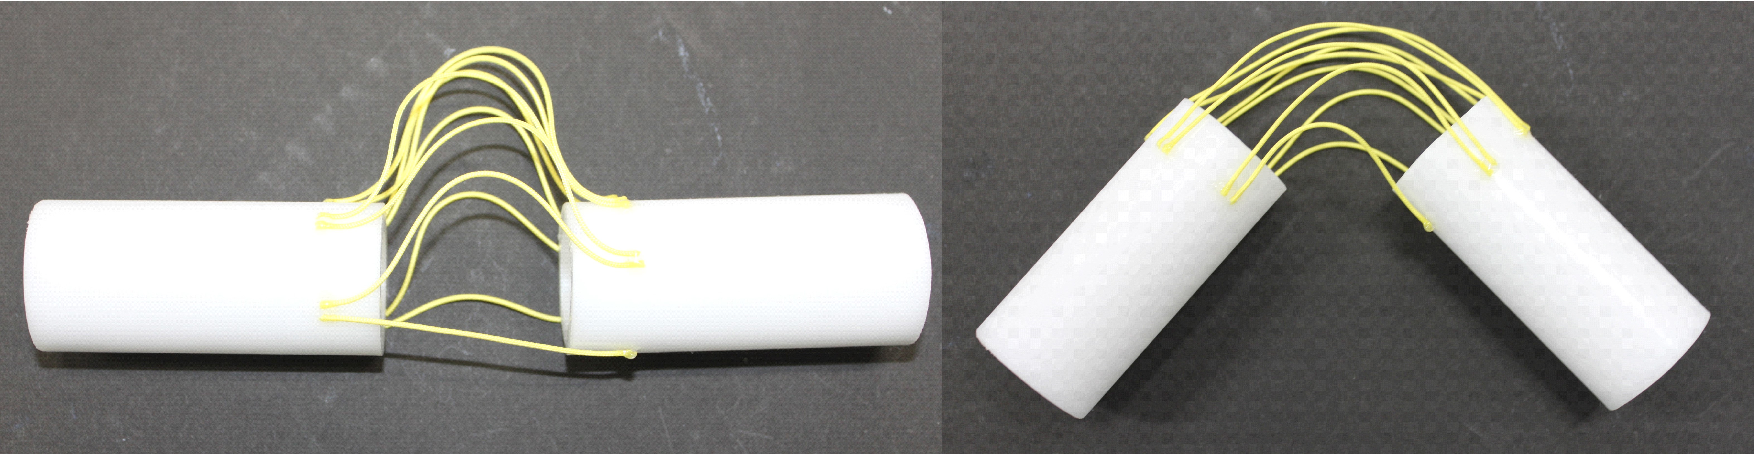
\includegraphics[width=70mm]{figure/目指す紐関節}
  \caption{Joint consisted of strings}
  \label{紐関節}
\end{figure}
\begin{figure}[h]
  \centering
  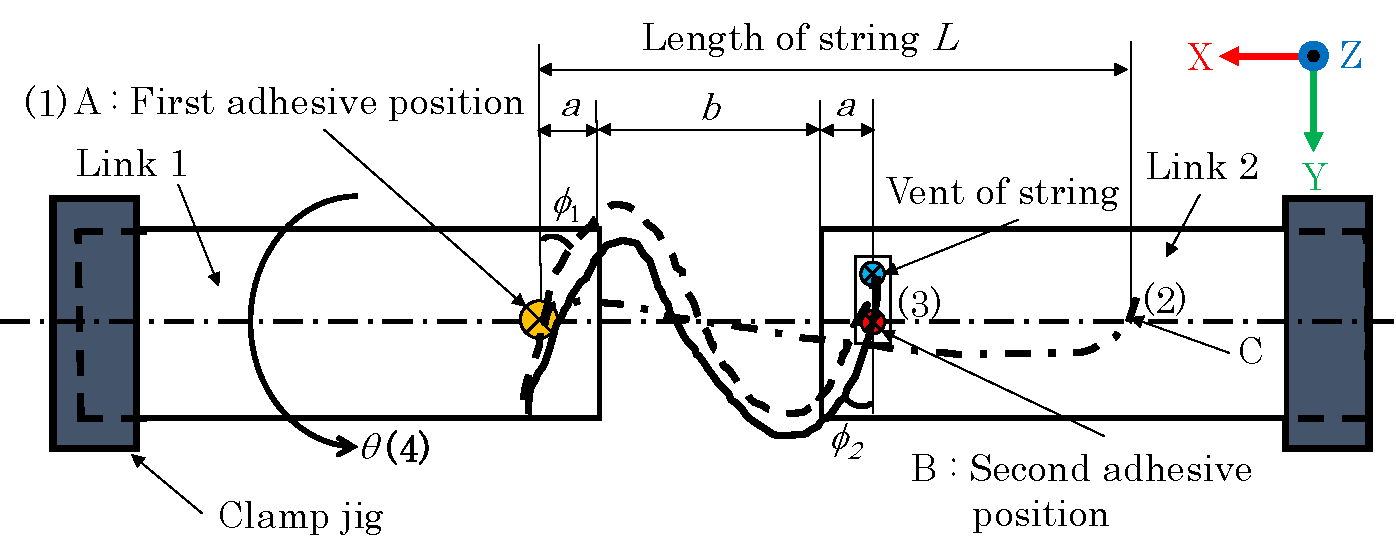
\includegraphics[width=70mm]{figure/abst用製造手法}
  \caption{Flow for connecting string}
  \label{製造手法}
\end{figure}

\section{実験方法}
実験には,直径は31mm,長さは90mmのPOM円柱をリンクとして使用し,紐は直径1.0mmのポリエステル素材のもの,接着剤は透明色の紫外線レジンを使用した.リンクはクランプ治具にボルトで挟み込んで固定する.クランプ後の2つの円柱の距離$b$を46mm,リンクの端から接着位置までの長さ$a$を10mm,線分ABの長さ$\delta$は48.3mmとする.
\par
実験手順を説明する.紐の長さ$L$を65~110mmの範囲において,5.0mm刻みに変化させる.また,それぞれの紐の長さ$L$でリンク1を5.0°の刻み角度において紐が目標の接着位置に到達する$\theta$を求める.ただし,$\theta$は0~180°と0~-180°の2つのパターンで回転させる.目標の接着位置は点Bにおける紐の角度$\phi_2$が$\pm{15}$°以内とする.目標の接着位置に入るリンク1の回転角度$\theta$の最小値$\theta_{min}$と最大値$\theta_{max}$を測定する.

\section{実験の結果と考察}
紐の長さ$L$と目標の接着位置に到達する角度$\theta_{min}$,$\theta_{max}$をそれぞれ3回試行し,平均したグラフを図\ref{実験結果}に示す.エラーバーは,角度$\theta_{min}$,$\theta_{max}$それぞれの最大値と最小値を示す.図\ref{実験結果}より,回転角度$\theta_{min}$は紐の長さ$L$に対して単調減少であったが,回転角度$\theta_{max}$は紐の長さ$L$=75mmまで増加した後,紐の長さ$L$=80mmからは単調減少となった.また,回転角度$\theta_{max}$と$\theta_{min}$の差を観察すると,紐の長さ$L$=75mmまでは増加傾向にあるが,それ以降は約90°の幅で前後している.全ての紐の長さ$L$に対して,目標の接着位置にくる回転角度$\theta_{max}$,$\theta_{min}$の差が約70°以上と大きい.よって,異なる長さ$L$の紐を安定して接着するためにはそれぞれの紐の長さ$L$における回転角度$\theta_{max}$,$\theta_{min}$の範囲内に回転角度を装置に入力することで,実際に接着が可能になると考えられる.

\section{結言}
本研究では,紐関節を製造できる装置を提案し,製作を行った. また,紐の長さ$L$と目標の接着位置に到達する角度$\theta_{min}$,$\theta_{max}$を実験により検証した.
\par
実験結果より,点A接着後の紐の角度$\phi_1$=0°における紐の長さ$L$とリンク1の回転角度$\theta_{max}$,$\theta_{min}$の差が約70°以上と大きいため,この範囲内に回転角度を指定することで実際に装置を用いて接着可能であることが分かった.

\begin{figure}[h]
  \centering
  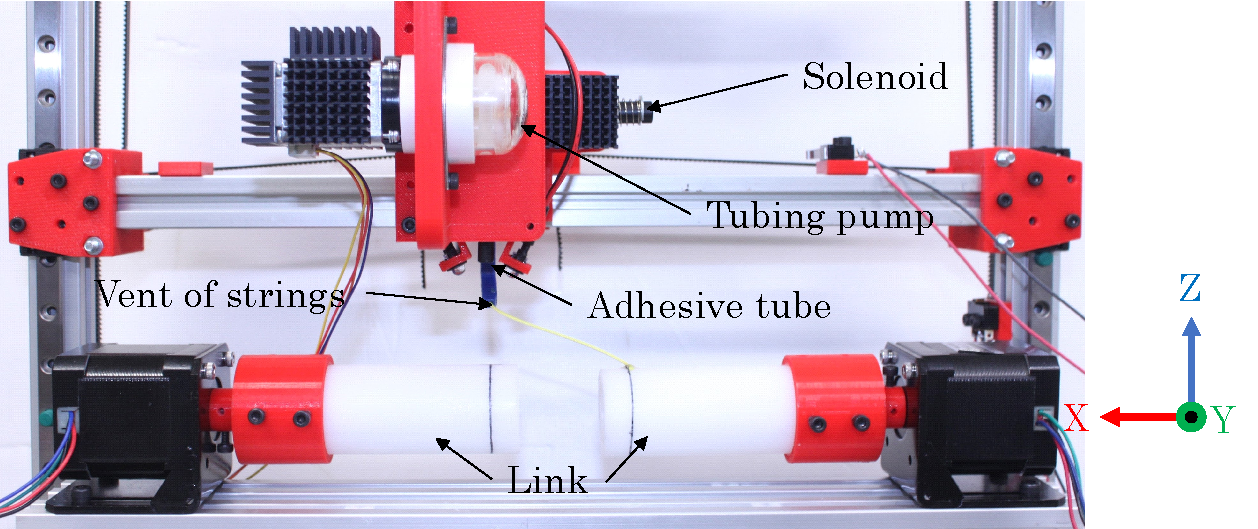
\includegraphics[width=78mm]{figure/abst用接続装置}
  \caption{Produced device}
  \label{接続装置}
\end{figure}

\begin{figure}[h]
  \centering
  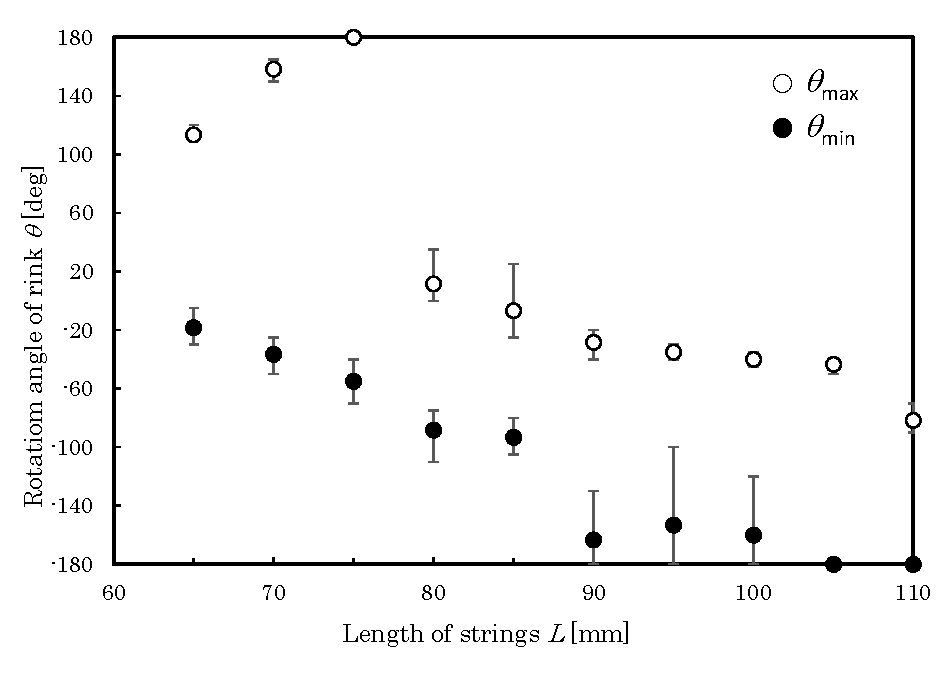
\includegraphics[width=77mm]{figure/実験結果}
  \caption{Experimental result}
  \label{実験結果}
\end{figure}